% !TeX program = latexmk
%%%
%%% LaTeX 2e (mostly) version of TTU thesis and dissertation format
%%% by Mike Renfro (renfro at tntech.edu) et al
%%%
%%% Basic instructions for document and formatting options are
%%% included inline throughout the .tex files -- read them thoroughly,
%%% and avoid changing anything other than what is specifically listed
%%% as editable.

%%% On the \documentclass line below, one thing you might need to
%%% change would be the font size. 10pt, 11pt, and 12pt are all
%%% accepted by the Graduate School, but your advisor and committee
%%% may be more restrictive. The default of 12pt should be fine unless
%%% you have a very large committee and a long thesis or dissertation title,
%%% which would overflow the approval sheet. You may also want to add the
%%% draft option, which will reformat your thesis to take up fewer sheets
%%% during the early editing process. Finally, you may want to add the
%%% copyrighted option, which will add a copyright page to the front matter.
\documentclass[11pt,oneside]{ttuthesis}

%%% For all notes below, let JOBNAME equal the base filename of this
%%% main .tex file for your thesis/dissertation (that is, this file you're
%%% reading right now). The macro \jobname has already been set to this value,
%%% and is used in several places below. There is no need to change this unless
%%% you decide to totally rearrange how various content and settings are stored.
%%%
%%% Go ahead and save this file under a new name (thesis-your-last-name.tex or
%%% thesis-your-ttu-username.tex, for example). That way, if you happen to
%%% update to a new version of the thesis files, your changes won't be
%%% overwritten. Also, make a new subdirectory in this directory named
%%% similarly (for example, thesis-your-last-name-content or
%%% thesis-your-ttu-username-content) to hold your chapters, figures, and other
%%% related items.

%%% Notes on adding other packages to your thesis:
%
% 1. The memoir class that ttuthesis.cls is based from already
%    emulates many packages' features. There is no need to load any of the
%    following packages at all---simply use their commands as if you'd already
%    loaded them:
%
%    appendix, array, booktabs, ccaption, chngcntr, crop, dcolumn, delarray,
%    enumerate, epigraph, framed, ifmtarg, ifpdf, index, makeidx, moreverb,
%    needspace, newfile, nextpage, pagenote, patchcmd, parskip, setspace,
%    shortvrb, showidx, tabularx, titleref, tocbibind, tocloft, verbatim,
%    verse.
%
% 2. The memoir class also provides functions equivalent to those in the
%    following packages, although it does not prevent you from loading them
%    via \usepackage:
%
%    fancyhdr, geometry, sidecap, subfigure, titlesec.
%
% 3. ttuthesis.cls automatically loads the following packages. There is
%    no need to re-load them in your own files:
%
%    hypcap, hyperref, ifthen, indentfirst, listings, memhfixc, nomencl,
%    refcount, rotating, ted.
%
% 4. For any remaining packages you need to load, some may need to be
%    loaded before hyperref, and some may need to be loaded after hyperref.
%    Add your entries to JOBNAME-packages-loaded-before-hyperref.sty and
%    JOBNAME-packages-loaded-after-hyperref.sty as appropriate.

%%% Your thesis or dissertation title. Insert line breaks manually
%%% with the \\ characters so that when printed, the title has an
%%% inverted pyramid format. If your title contains Greek letters,
%%% superscripts, subscripts, or other typography that can't be
%%% rendered as a PDF string, use the command
%%% \title{\texorpdfstring{TeX title}{PDF title}} instead.
\title{Data-Driven Assessment of Network-Based Anomaly Detection Systems Protecting Cyber-Physical Systems}

%%% Your name, as registered at the university.
\author{Robert E. Gillen}

%%% This example and style file was designed to render into a PDF file
%%% rather than DVI or Postscript, and for all cross-references (to
%%% specific chapters, pages, equations, references, etc.) to be
%%% hyperlinks in that PDF. The hyperref package handles the
%%% hyperlinks, and also the basic metadata for the PDF, such as the
%%% author, keywords, etc.
%%%
%%% ttuthesis.cls automatically fills out the fields for pdfauthor and
%%% pdftitle. The pdfkeywords and pdfsubject fields are optional, but
%%% may be useful in the future if we do an electronic archive of
%%% theses and dissertations and want to make it easier to search. If
%%% you don't fill out accurate subject and keywords fields, please
%%% remove or comment the following hypersetup command entirely.
%%%
\hypersetup{
  pdfsubject={Format and style rules for theses and dissertations at Tennessee Technological University},
  pdfkeywords={thesis, dissertation, style guide}
}

%%%
%%% Other information relevant to the front matter of your thesis.
%%%

%%% Your abstract.
\abstract{%
  My thesis has an abstract. Here it is.
}

%%% Is this document and thesis or a dissertation?
\doctype{Dissertation}

%%% Your planned degree
\degree{Doctorate of Philosophy}

%%% Your major. Engineering PhD students would just put Engineering
%%% here, not a specific department's name.
\department{Engineering}

%%% The month and year of your graduation.
\graduationmonth{December}
\graduationyear{2019}

%%% The text of your dedication page, if you have one.
\dedication{%
  \begin{center}
    This thesis is dedicated to my parents \\
    who have given me invaluable educational opportunities.     
  \end{center}
}

%%% The text of your acknowledgments page.
\acknowledgments{%
  Appreciation is extended to my advisor and other committee members.
}
%%%
%%% Information about your committee.
%%%
%%% Note: you may have to switch to a smaller font if your
%%% thesis/dissertation title is very long and your committee is very large.
%%% Using a 10pt font, a title seven lines long only allows for six people
%%% on the committee (including chairs and cochairs). A title two lines long
%%% allows for up to nine people on the committee (including chairs and
%%% cochairs).

%%% First, who is your committee chair?
\committeechair{Steven Scott}

%%% Second, does your committee have a single chair, or two cochairs?
%%% If you have two cochairs, use one name in \committeechair, and the
%%% second name in \committeecochair. If you have no cochair, leave the
%%% \committeecochair command commented out.
%\committeecochair{Cochair's Name}

%%% Third, what are the names of your committee members?
\committeemembers{Adam Anderson, William Eberle, Mike Rogers, Sheikh Ghafoor}

\begin{document}

%%%
%%% Typesetting your document's front matter. Most of this is automated.
%%%
%%% Abstract page, title page: mandatory, automatically added to all
%%% theses and dissertations. Use the \abstract, \title, \author, \doctype,
%%% \degree, \department, \graduationmonth, and \graduationyear commands
%%% above to edit the page content. The page format and location is fixed,
%%% and cannot be edited.
%%%
%%% Copyright page: optional, automatically added to all theses and
%%% dissertations with copyrighted in the \documentclass options above. The
%%% page format and location is fixed, and cannot be edited.
%%%
%%% Approval page: mandatory, automatically added to all theses and
%%% dissertations. Placed immediately after the copyright page (if present)
%%% or the title page (if no copyright page is present).  The page format
%%% and location is fixed, and cannot be edited.
%%%
%%% Dedication page: optional, automatically added to all theses and
%%% dissertations with a \dedication command. Placed immediately after the
%%% approval page. The \dedication command defines the content of the 
%%% dedication page. The page format and location is fixed, and cannot be
%%% edited.
%%%
%%% Acknowledgments page: optional, automatically added to all theses and
%%% dissertations with a \acknowledgments command. Placed immediately after the
%%% dedication page (if present) or the approval page (if no dedication page
%%% is present). The \acknowledgments command defines the content of the 
%%% acknowledgments page. The page format and location is fixed, and cannot be
%%% edited.

%%% The table of contents and lists of figures, tables, etc. Except
%%% for commenting out the lists of tables, figures, or other elements
%%% missing from your document, you shouldn't need to change any of
%%% the table of contents commands.
\begin{Spacing}{1}
\tableofcontents*  % Leave the * after this command to keep the table of
                   % contents from appearing in the table of contents
\listoftables      % Tables
\listoffigures     % Figures
\lstlistoflistings % Program Listings, from the listings package
%%% If you want to rename your list of symbols, edit the
%%% \renewcommand{\nomname} command accordingly.
\renewcommand{\nomname}{LIST OF SYMBOLS}
\printnomenclature % Symbols
\end{Spacing}

%%% Leave the \mainmatter and command alone. This resets the page numbering
%%% and styles from what's appropriate for the front matter to what's
%%% appropriate for the body of your thesis/dissertation.
\mainmatter

%%% Edit the \include commands below to match the base filenames of
%%% your chapter files. Do *not* add a .tex extension to the filename
%%% -- chapter1.tex is included with a \chapter{The Essentials}
\label{chap:TheEssentials}

\section{Purpose of the Guide}
\label{sec:PurposeOfTheGuide}

This guide is designed to be a basic source of information for
the\-sis/dis\-ser\-ta\-tion preparation. It establishes the technical
parameters within which you should work, such as quality of paper,
number of copies to be submitted, margins, and the sequence of pages
within the manuscript. Since most of you will publish during and after
your graduate education, this guide encourages the use of leading
professional publications to help establish specific formatting
convention. You are encouraged to use publications within your
field---journals and textbooks---to assist you in establishing
bibliographic form, use of number, and other conventions that are
discipline oriented.  However, the application of this theory is not
simple. You must understand the various elements of a manuscript and
general publication formatting requirements in academic publishing.
Although knowledge and use of publication formatting is essential, the
regulations established by this guide always take precedence.

You should use style handbooks such as the most recent editions of the
\textit{MLA Handbook for Writers of Research Papers} (English)
\cite{gibaldi1988}, \textit{Publication Manual of the American
  Psychological Association} (Education) \cite{apa1983}, \textit{CBE
  Style Manual (Biology)} \cite{cbe1983}, \textit{Form and Style}
(Arts \& Sciences, Engineering, Education) \cite{campbell1990},
\textit{The Chicago Manual of Style} \cite{chicago1982}, and
\textit{Harbrace College Handbook} \cite{hodges1990} as resources for
basic style and grammar. In contrast, you should never use previously
accepted theses and dissertations as the final guide to style.
Examples taken from other theses may be out of context or may be
incorrect. The existence of a particular style or usage in a
previously accepted thesis does not establish a precedent for its
continuation.
% The following two nomenclature entries are intended for the thesis manual.
% Best practice is to add \nomenclature commands with first use of a term.
\nomenclature{MLA}{Modern Language Association}
\nomenclature{CBE}{Council of Biological Editors}

By accepting your thesis or dissertation and awarding the degree,
Tennessee Technological University places its academic reputation on
the line. The content of your manuscript is carefully evaluated by
experts in your field. The format requirements presented in this guide
are imposed to ensure an appropriate academic appearance of your
manuscript.


\section{Ethical Standards}
\label{sec:EthicalStandards}

Since conferral of a graduate degree implies professional integrity
and knowledge of scholarly methods, there are three areas in which you
as a graduate student should be particularly cautious:

\begin{itemize}
\item proper acknowledgment of cited works
\item the proper use of copyrighted material
\item the proper reporting of work where research compliance is required
\end{itemize}

\subsection{Plagiarism}
\label{sec:Plagiarism}

\textit{Merriam-Webster's Collegiate Dictionary} \cite{webster1993}
defines plagiarism as ``steal\-[ing] and pass\-[ing] off ideas or
words of another as one's own'' and ``the use of a created production
without crediting the source.'' ``You must acknowledge all material
quoted, paraphrased, or summarized from any published or unpublished
work.  Failing to cite a source, deliberately or accidentally, is
plagiarism'' \cite[424]{webster1993}. If you use the exact words of
your source, they must be enclosed in quotation marks and the source
cited; if you do not use the exact words but paraphrase or summarize
the source, it still must be cited.  When involved in collaborative
research, you should exercise extreme caution to avoid questions of
plagiarism. If in doubt, check with your major professor and the
Graduate School about the project. Plagiarism will be investigated
when suspected and prosecuted if established.


\subsection{Copyright}
\label{sec:Copyright}

If you use copyrighted material in a limited way, it is usually
unnecessary to seek permission to quote. If, however, you use material
from a copyrighted work to the extent that the rights of the copyright
owner might be violated, you must obtain permission of the owner. In
determining the extent of a written work that may be quoted without
permission, you should consider the proportion of the material to be
quoted in relation to the substance of the entire work. According to
\textit{The Chicago Manual of Style} \cite{chicago1982}, ``A few lines
from a sonnet, for instance, form a greater proportion of the work
than do a few lines from a novel. Use of anything in its entirety is
hardly ever acceptable'' (p. 124). In no case should you copy a
standardized test of similar material and include it in a
the\-sis/dis\-ser\-ta\-tion without written permission. According to
Circular 21 (Reproduction of Copyrighted Works by Educators and
Librarians, p. 11) \cite{loc1988}, ``\textellipsis{}the following
shall be prohibited: \textellipsis{} There shall be no copying of or
from works intended to be `consumable' in the course of study or of
teaching.  These include workbooks, exercises, standardized tests and
test booklets and answer sheets and like consumable material.'' The
publisher usually has the authority to grant permission to quote
excerpts from the copyrighted work or can refer requests to the
copyright owner or designated representative.  The copyright owner may
charge for permission to quote. You should credit permissions with the
acknowledgments, and the source should appear in the
Bibliography\footnote{Some fields alternatively use Literature Cited,
  References, or Works Cited.}.


\subsection{Federal and State Regulations}
\label{sec:FederalAndStateRegulations}

Compliance with federal and state regulations governing the use of
human subjects, animal care, radiation, legend drugs, recombinant DNA,
or the handling of hazardous materials/wastes in research is monitored
by a number of regulatory agencies. Because of these regulations,
research compliance is another area of importance to you as a graduate
student and to the conduct of your research. Tennessee Technological
University requires you to verify that you have complied with the
appropriate approval procedure(s) prior to the initiation of the
thesis- or dissertation-related research, if approval is relevant to
the research. If your research involves any of the areas mentioned
above, you should determine what compliance is required by the school
(available in the Office of Research).


\section{Definitions}
\label{sec:Definitions}


\subsection{Typeface or Font}
\label{sec:DefTypefaceOrFont}

These terms apply to all the features available within a ``type''
family. For many printers, typeface includes bold, italic, and the
various sizes of any named type (Helvetica, Times Roman, New York,
Geneva, etc.).


\subsection{Text}
\label{sec:DefText}

In the discussion of formatting, text is used as a generic term to
designate the main body of the the\-sis/dis\-ser\-ta\-tion and to
distinguish this element from preliminary pages, references, tables,
figures, and appendices.


\subsection{Preliminary Pages}
\label{sec:DefPreliminaryPages}

Sometimes called ``front matter,'' preliminary pages serve as a guide
to the contents and nature of the manuscript \cite{chicago1982}. The
approval or acceptance sheets, as part of the preliminary pages,
confirm acceptance by the committee members acting for the department,
and the Dean of Graduate Studies, acting for the university or
college.


\subsection{Table}
\label{sec:DefTable}

A table consists of numbers, words, or both, and presents information
that is separated into columns. Tabular information allows you, the
author, to convey information to a reader in a structured format.


\subsection{Figure}
\label{sec:DefFigure}

Any diagram, drawing, graph, chart, map, photograph, or material that
does not fit into the restricted format for a table is a figure.
Figures generally show relationships or illustrate information rather
than present precise data.


\subsection{Appendix}
\label{sec:DefAppendix}

An appendix is generally a ``catch-all'' for supplementary material to
the the\-sis/dis\-ser\-ta\-tion. In some cases, tables and/or figures
are placed in an appendix to avoid interrupting the text. An example of an appendix can be seen in Appendix~\ref{chap:sample_tables}.

%%% Local Variables: 
%%% mode: latex
%%% TeX-master: "thesis"
%%% End: 
 command.
\chapter{Introduction and Literature Review}

This chapter contains my introduction and literature review. We might define
$m$\nomenclature{$m$}{Mass} as the mass of some object. We might also cite a
book as~\cite{lacava1992}. See Figure~\ref{fig:panel-al4} or
Table~\ref{table:amplitude} for more information.
\begin{figure}[tbp]
\centering
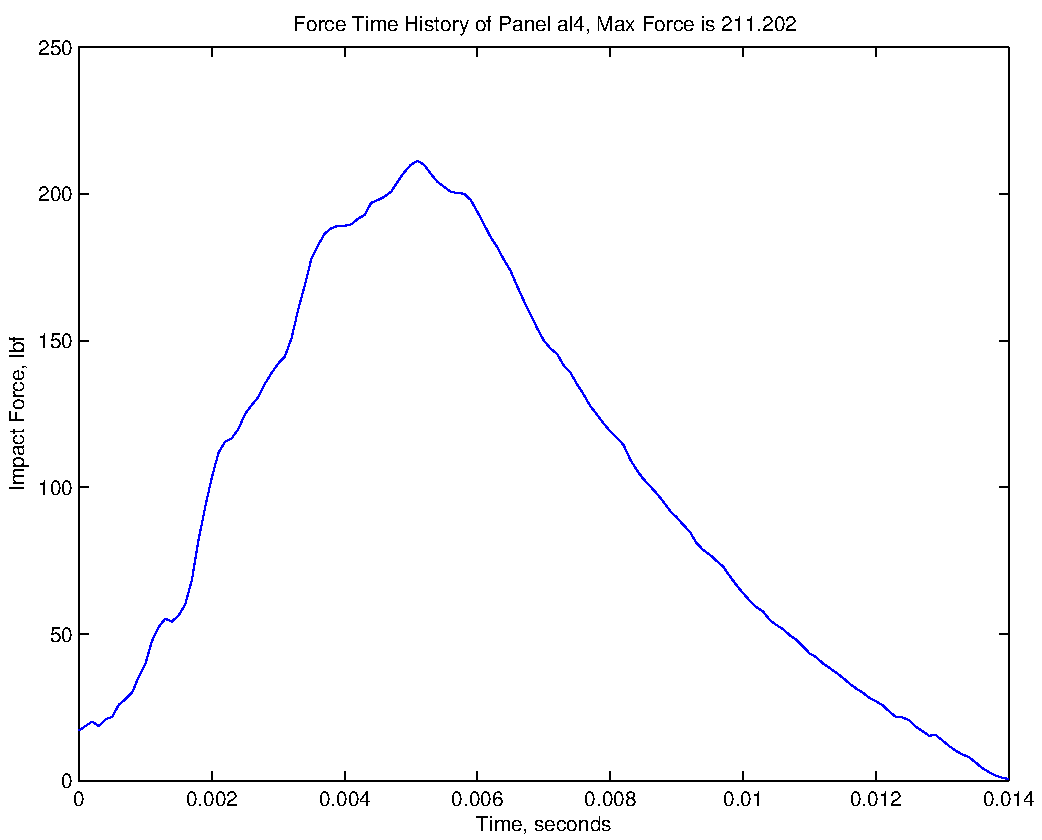
\includegraphics[width=\textwidth]{al4-1}
\caption{Force Time History of Panel ``al-4''\label{fig:panel-al4}}
\end{figure}
\begin{table}
\caption{GNU Radio Amplitude and Corresponding Voltages\label{table:amplitude}}
\centering
% \begin{tabular}{SSS}
% \toprule
% % text headers often need to be enclosed in braces to keep siunitx from
% % mis-interpreting them as units
% {GNU Radio Amplitude} & {Oscilloscope} & {Calculated Power} \\ 
%  & \si{\mvrms} & \si{\dbm} \\
% \midrule
% 0.1 &  28.5 & -8.946 \\
% 0.2 &  57.1 & -5.928 \\
% 0.3 &  85.2 & -4.190 \\
% 0.4 & 116.5 & -2.831 \\
% 0.5 & 140.4 & -2.021 \\
% 0.6 & 167.5 & -1.255 \\
% 0.7 & 196.9 & -0.552 \\
% 0.8 & 227.3 &  0.071 \\
% 0.9 & 257.2 &  0.608 \\
% 1.0 & 273.9 &  0.881 \\
% 1.5 & 273.6 &  0.876 \\tokentoken
% 2.0 & 273.6 &  0.876 \\
% 2.5 & 273.4 &  0.873 \\
% 3.0 & 274.1 &  0.884 \\
% 3.5 & 273.2 &  0.870 \\
% 4.0 & 269.7 &  0.814 \\
% 4.5 & 271.6 &  0.845 \\
% 5.0 & 273.7 &  0.878 \\
% \bottomrule
% \end{tabular}
\end{table}
%\include{\jobname-content/analytical}
%\include{\jobname-content/experimental}
%\include{\jobname-content/results}
%\include{\jobname-content/conclusions}

%%% Bibliography settings
\renewcommand{\bibname}{References}
%%% If you're using BibTeX, fill out the following two commands with the name
%%% of your .bib file and the name of your .bst file. Otherwise, comment them
%%% out:

\bibliography{\jobname-content/\jobname}
\bibliographystyle{ttunatbib-mwr}
%\bibliographystyle{plain}

%%% If you're doing your bibliography manually, then uncomment the
%%% following lines and enter your bibliography entries below:


%%%
%%% Appendices settings
%%%

%%% Does your thesis have one appendix, or multiple appendices?
%%% Uncomment or comment each of the next two lines accordingly.
\renewcommand{\appendixtocname}{Appendix} % I have only one appendix
%\renewcommand{\appendixtocname}{Appendices} % I have multiple appendices

%%% If you have any appendices on your thesis, leave the \appendix and
%%% command alone. It resets the ToC style to label your appendices by
%%% letter rather than number, and typesets the required separation page
%%% between the Appendices and the main body text. If you have no
%%% appendices, comment the \appendix command.
\appendix

%%% Edit the \include commands below to match the relative path and base
%%% filenames of your appendix files. Do *not* add a .tex extension to the
%%% filename -- appendix-a.tex is included with a \chapter{Sample Tables}
\label{chap:sample_tables}

\begin{table}[tbp]
  \caption{Lin Plate and Incremental Loading Method Deflections Along Free Edge in Inches}
  \label{tab:LinPlate}
  \centering
  \begin{tabular}{rrrrrr} \hline
    Total & Position & \multirow{3}{*}{Lin Plate} & \multicolumn{3}{c}{Deflections} \\
    Load & X-axis & & \multicolumn{3}{c}{Incremental Loading Method} \\
    (lbs) & (in) & & 1,49,72 & 10,49,72 & 20,169,288 \\
    \hline
    \\
    0.722 & 1.0 & -.04 & -.043 & -.046 & -.047 \\
    \\
    & 2.0 & -.16 & -.166 & -.165 & -.166 \\
    \\
    & 3.0 & -.36 & -.349 & -.331 & -.333 \\
    \\
    & 4.0 & -.56 & -.574 & -.531 & -.533 \\
    \\
    & 5.0 & -.78 & -.828 & -.753 & -.757 \\
    \\
    & 6.0 & -1.04 & -1.100 & -.992 & -1.000 \\
    \\ \hline
  \end{tabular}
\end{table}

\begin{table}[tbp]
  \caption{Means and standard errors of depths occupied by threadfin shad, alewife, and walleye in Dale Hollow Reservoir, Tennessee. Mean depths that share the same letter are not significantly different (Tukey's test; $P>0.05$)}
  \label{tab:FishDepths}
  \centering
  \begin{tabular}{llrrr} \hline
    & & & \multicolumn{2}{c}{DEPTH (m)} \\ \cline{4-5}
    SEASON & SPECIES & N & MEAN & SE \\ \hline
    Summer 1990 & Threadfin shad & 2043 & $6.6^{\textrm{a}}$ & 0.08 \\
    Summer 1990 & Alewife & 816 & $12.5^{\textrm{b}}$ & 0.13 \\
    Summer 1990 & Walleye & 22 & $10.3^{\textrm{c}}$ & 0.62 \\
    \\
    Fall 1990 & Threadfin shad & 283 & $6.7^{\textrm{a}}$ & 0.29 \\
    Fall 1990 & Alewife & 447 & $9.0^{\textrm{b}}$ & 0.33 \\
    Fall 1990 & Walleye & 26 & $10.5^{\textrm{b}}$ & 0.96 \\
    \\
    Winter 1990 & Threadfin shad & 72 & $3.0^{\textrm{a}}$ & 0.34 \\
    Winter 1990 & Alewife & 395 & $7.3^{\textrm{b}}$ & 0.31 \\
    Winter 1990 & Walleye & 13 & $10.5^{\textrm{b}}$ & 1.63 \\
    \\
    Spring 1991 & Threadfin shad & 749 & $2.7^{\textrm{a}}$ & 0.07 \\
    Spring 1991 & Alewife & 689 & $4.5^{\textrm{b}}$ & 0.08 \\
    Spring 1991 & Walleye & 3 & $4.3^{\textrm{a}}$ & 1.67 \\
    \\
    Summer 1991 & Threadfin shad & 151 & $10.5^{\textrm{a}}$ & 0.13 \\
    Summer 1991 & Alewife & 1251 & $12.3^{\textrm{b}}$ & 0.09 \\
    Summer 1991 & Walleye & 10 & $12.2^{\textrm{a}}$ & 1.16 \\
    \\
    Fall 1991 & Threadfin shad & 39 & $4.4^{\textrm{a}}$ & 0.47 \\
    Fall 1991 & Alewife & 66 & $6.3^{\textrm{b}}$ & 0.48 \\
    Fall 1991 & Walleye & 10 & $10.1^{\textrm{c}}$ & 0.77 \\
    \\ \hline
  \end{tabular}
\end{table}

\begin{sidewaystable}[tbp] 
  \caption{Meristic Characters used in Distinguishing Redeye Bass, Smallmouth Bass, and Meristic Hybrids from Roaring River, Tennessee, 1988}
  \label{tab:MeristicCharacters}
  \centering
  \begin{tabular}{lccc} \hline \hline
    \\
    & \textit{Micropterus coosae} & Meristic Hybrids & \textit{Micropterus dolomieui} \\
    & $n=32$ & $n=20$ & $n=35$ \\\
    & $x\pm$ SD & $x\pm$ SD & $x\pm$ SD \\
    Meristic & (range) & (range) & (range) \\
    \\ \hline
    \\
    Lateral line scales & $66.9 \pm 2.6$ & $71.4 \pm 1.6$ & $74.1 \pm 2.4$ \\
    & (61--71) & (70--75) & (69--79) \\
    \\
    Scales above lateral line & $8.7 \pm 0.5$ & $9.9 \pm 1.0$ & $11.8 \pm 0.7$ \\
    & (8--10) & (8--12) & (11--13) \\
    \\
    Scales below lateral line & $15.9 \pm 1.8$ & $17.5 \pm 2.4$ & $21.8 \pm 2.4$ \\
    & (11--19) & (13--21) & (14--25) \\
    \\
    Anal rays & $10.1 \pm 0.7$ & $10.7 \pm 0.7$ & $11.1 \pm 0.4$ \\
    & (9--12) & (9--12) & (10-12) \\
    \\
    Pyloric cacea & $10.8 \pm 2.0$ & $11.7 \pm 0.7$ & $11.1 \pm 0.4$ \\
    & (7--17) & (10--14) & (10--16) \\
    \\
    Meristic index & $112.2 \pm 3.7$ & $119.1 \pm 3.6$ & $131.6 \pm 4.2$ \\
    & (102--120) & (115--125) & (123--140) \\
    \\ \hline
  \end{tabular}

  \parbox{\textheight}{Source: William D. Crumby, ``Growth Dynamics of
    an Introduced Population of Redeye Bass in a North-Central
    Tennessee Stream.''  Master of Science Thesis in Biology,
    Tennessee Technological University, August 1987.}
\end{sidewaystable}

%%% Local Variables: 
%%% mode: latex
%%% TeX-master: "thesis"
%%% End: 

%%% command. Obviously, if your thesis has no appendices, then comment them
%%% all.
%\chapter{Code Listings}

\begin{Spacing}{1}
\lstset{basicstyle=\ttfamily\small,commentstyle=\color{red}}
\begin{lstlisting}[language=matlab,numbers=left,stepnumber=5,numberfirstline=false,firstnumber=1,caption={A Very Old MATLAB Function},label={lst:myfft}]
function [X,f]=myfft(x,t)
% myfft - An FFT function with usable output
%
% Usage: [X,f] = myfft(x,t)
%
% Where:     x is some time-domain signal
%            t is the time axis for x
%
%  Note: t must be an evenly-spaced vector
%        f is in units of Hz (multiply by 2pi to get rad/s)
n_points=2^(floor(log(length(x))/log(2)));
fftX=2*fft(x,n_points)/length(t);
fftX(1)=[];
dt=t(2)-t(1);
maxfreq=1/(2*dt);
nyquist = 1/2;
f = (1:n_points/2)/(n_points/2)*nyquist/dt;
X = fftX(1:n_points/2);
\end{lstlisting}
\end{Spacing}


%%% Edit the \vita command below to match the relative path and base
%%% filename of your vita. Do *not* add a .tex extension -- vita.tex is
%%% included with a \vita{vita} command.
\vita{\jobname-content/vita}

\end{document}
